\documentclass{article}
\usepackage{graphicx}
\usepackage{listings}
\usepackage{float}
\usepackage[croatian]{babel}
\usepackage{color}
\usepackage{svg}
\usepackage[utf8]{inputenc}
\usepackage{amssymb}
\usepackage{amsmath}
\usepackage{comment}
\usepackage{titlesec}
\usepackage{minted}
\usepackage{hyperref}
\graphicspath{ {./images/} }
\usepackage{a4wide}
\usepackage[top=60pt,bottom=60pt,left=100pt,right=100pt]{geometry}
\usepackage{caption}

\begin{document}

\title{\textbf{Organizacija logistike oružanih snaga Bosne i Hercegovine u PDDL jeziku}}
\author{\textbf{Tim 17:}\\\textit{Vedad Gaštan}\\\textit{Aldin Velić}\\\textit{Irhad Žiga}\\\textit{Kerim Hajdar}\\\\\textbf{Predmetni profesor/i}:\\\textit{Doc. dr Senka Krivić}\\\textit{Doc. dr Kenan Šehić}}
\date{Juni 2024}

\topskip200pt
\maketitle
\topskip0pt
\newpage
\tableofcontents
\newpage
\section{Uvod}
Logistika je ključan faktor u funkcionisanju svih oružanih snaga savremenog doba, jer značajno poboljšava efikasnost i pravovremenost snabdjevanja jedinica svim neophodnim resursima, od municije i goriva do medicinske i zaštitne opreme.


\subsection{Motivacija}
Naš tim je za temu konkretno odabrao organizaciju logistike oružanih snaga države Bosne i Hercegovine. Naš zadatak je da u PDDL jeziku izvršimo modeliranje već postojećeg sistema logistike oružanih snaga BiH kojeg smo predformirali na osnovu informacija koje smo mogli pronaći na internetu. Treba napomenuti da nije moguće tek tako pronaći sve moguće istinite informacije vezane za oružane snage Bosne i Hercegovine koje su neophodne za modeliranje koje planiramo napraviti, tako da ćemo u nastavku ovog rada uzimati zdravo za gotovo ili proizvoljno definisati neke pojmove koji su nam potrebni ili za koje mislimo da će nam biti od koristi.
\\PDDL je formalni jezik koji na efikasan način omogućava modeliranje i kreiranje optimalnih logističkih planova.
\\U ovom radu, cilj je pružiti uvid u mogućnosti primjene PDDL jezika u vojnoj logistici, a glavni fokus će biti stavljen na definisanju domena i problema u PDDL-u koji odgovaraju različitim logističkim scenarijima. 
\subsection{Opis problema}
Logistika oružanih snaga Bosne i Hercegovine suočava se sa nizom izazova koji znatno otežavaju njenu organizovanost kao što su:
\begin{itemize}
    \item Geografski izazovi
    \\Bosna i Hercegovina je zemlja sa raznolikim geografskim terenom što može otežavati transport i distribuciju potrebne opreme, pogotovo u udaljenim i teško pristupačnim područjima. 
    \item Infrastrukturni problemi
    \\Putna mreža u Bosni i Hercegovini je generalno nerazvijena zbog nedostatka kvalitetnih puteva, mostava i tunela, kao i zbog loše željezničke infrastukture koja je poprilično zastarjela, što dodatno komplikuje logističke operacije.
    \item Nedovoljna tehnološka opremljenost
    \\Nedostatak savremenih sistema za praćenje i upravljanje logistikom, kao i zastarjela oprema i vozila smanjuju efikasnost logistike.
    \item Resursna ograničenja
    \\Finansijski problemi impliciraju nemogućnost nabavljanja dovoljne količine potrebne opreme i zaliha, što direktno utiče na operativnu spremnost jedinica.
\end{itemize}
Možemo zaključiti da svi prethodno navedeni problemi predstavljaju veoma kompleksnu problematiku u koju ne možemo duboko zalaziti, ali donekle ćemo ih pokušati riješiti uspostavljanjem jednostavnijeg modela logistike u PDDL jeziku.
\\Oružane snage Bosne i Hercegovine su strukturisane na sledeći način:
\begin{itemize}
    \item 4. pješadijska brigada
    \item 5. pješadijska brigada
    \item 6. pješadijska brigada
    \item Brigada taktičke podrške
    \item Brigada zračnih snaga\\
\end{itemize}
Sada ćemo tabelarno predstaviti svu opremu kojom oružane snage raspolažu tako što ćemo ih podijeliti u kategorije prema vrsti:\\\\
\begin{tabular}{ |p{3cm}|p{2cm}|p{2cm}|  }
\hline
\multicolumn{3}{|c|}{Oprema oružanih snaga BiH} \\
\hline
Vrsta opreme& Domaća proizvodnja &Uvoz \\
\hline
Artiljerija & \checkmark & \\
Telekomunikacijska oprema & \checkmark &  \\
Zaštitna oprema & \checkmark &  \\
Eksplozivi    & \checkmark &  \\
Puške & \checkmark &  \\
Municija & \checkmark &    \\
Dodatna oprema & \checkmark &  \\
Napredni eksplozivi &  & \checkmark \\
Oklopna vozila &  & \checkmark \\
Tenkovi &  & \checkmark \\
Helikopteri &  & \checkmark \\
Borbeni avioni &  & \checkmark \\
Avioni presretači &  & \checkmark \\
\hline
\end{tabular}
\\\\Treba napomenuti da uvozimo samo ono što ne proizvodimo, a na taj način postižemo racionalno korištenje finansijskih resursa.
\\Sledeće domaće fabrike su zadužene za proizvodnju pomenute opreme: BINAS-DD, Čajevac, RZT, Igman, TRZ, Orao, Vitezit, Pretis, Kosmos i BNT
\\Svaka brigada uzima sebi opremu koja im je potrebna. Sledeća tabela predstavlja raspodjelu opreme po brigadama:\\\\
\begin{tabular}{ |p{3cm}|p{3cm}|p{3cm}|p{3cm}|  }
\hline
\multicolumn{4}{|c|}{Raspodjela opreme oružanih snaga BiH po brigadama} \\
\hline
Vrsta opreme& Pješadijske brigade & Brigada taktičke podrške & Brigada zračnih snaga \\
\hline
Artiljerija & \checkmark &  & \\
Telekomunikacijska oprema & \checkmark & \checkmark & \\
Zaštitna oprema & \checkmark & \checkmark & \\
Eksplozivi & \checkmark &  & \\
Municija & \checkmark &  & \\
Dodatna oprema & \checkmark & \checkmark & \\
Napredni eksplozivi &  & \checkmark & \\
Oklopna vozila & \checkmark &  & \\
Tenkovi & \checkmark &  & \\
Helikopteri &  &  & \checkmark \\
Borbeni avioni &  &  & \checkmark \\
Avioni presretači &  &  & \checkmark \\
Puške & \checkmark & & \checkmark \\
\hline
\end{tabular}
\\\\Oprema se smješta u neka od 3 moguća skladišta kojim oružane snage raspolažu. Također, vojska posjeduje 8 kamiona kojim dostavljaju opremu do brigada. Vrijedi napomenuti da smo broj kamiona i skladišta proizvoljno definisali jer ne možemo pronaći tačnu informaciju o tome na internetu.
\\Također, treba napomenuti da oružane snage Bosne i Hercegovine zapravo ne raspolažu određenom opremom koju smo prethodno naveli, kao što su npr. borbeni avioni i avioni presretači, ali smo ih dodali na listu opreme koju uvozimo u svrhu podizanja cjelokupnog nivoa opremljenosti oružanih snaga koji je veoma skroman, što smo ranije i spomenuli.
\\Naš cilj je da uspostavimo uspješno snabdjevanje svake od brigada potrebnom opremom, a u nastavku ćemo predložiti rješenje koje je modelirano u PDDL jeziku.
\newpage
\section{Predloženo rješenje}
Testiranjem se došlo do zaključka da implementacije finalnog modela bez testiranja uspješnosti jednostavnijih modela dovodi do značajno otežanog pronalaska rješenja. Kako je teško odjednom formirati konačan kod, ovaj ćemo postupak raditi u tri etape.
\begin{enumerate}
    \item Modeliranje najjednostavnije logistike - jedan pješadijska brigada, jedna fabrika, jedno skladište i jedan kamion.
    \item Usložnjavanje modela - dodavanje svih fabrika, jednostavnih pješadijskih brigada, dodatnih kamiona, skladišta i sve opreme.
    \item Finalni model - Dodavanje složenijih brigada i uvoza opreme.\\
\end{enumerate}

\Large
\noindent
\textbf{Model 1}
\\~\\
\normalsize 
Počnimo od najjednostavnijeg modela ovog problema. Uzmimo da imamo samo jednu pješadijsku brigadu, jednu fabriku koja proizvodi vojnu opremu, jedno skladište i jedan kamion. PDDL kod koji bi trebao biti u stanju pronaći potrebne korake da se vojna oprema dobremi do pješadijske brigade je sljedeći:
\\~\\
\textbf{\textit{domain.pddl}}
\begin{verbatim}
(define (domain vojna-logistika-minimal)
    (:requirements :strips :typing)
    (:types
        division factory warehouse good truck fuel
    )
    (:constants
        Pjesadijska-brigada-4 - division
        Factory1 - factory
        Warehouse1 - warehouse
        Artillery1 - good
        Truck1 - truck
        Fuel - fuel
    )
    (:predicates
        (produced ?f - factory ?g - good)
        (transported ?t - truck ?w - warehouse ?g - good)
        (stored ?w - warehouse ?g - good)
        (consumed ?d - division ?g - good)
        (truck_available ?t - truck)
        (division_needs ?d - division ?g - good)
    )
    (:action produce_goods
        :parameters (?f - factory ?g - good)
        :precondition (not (produced ?f ?g))
        :effect (produced ?f ?g)
    )
    (:action transport_goods
        :parameters (?t - truck ?w - warehouse ?g - good)
        :precondition (and (produced Factory1 ?g) (truck_available ?t))
        :effect (and (transported ?t ?w ?g) (stored ?w ?g) 
            (not (truck_available ?t)))
    )
    (:action consume_goods
        :parameters (?d - division ?g - good ?w - warehouse)
        :precondition (and (stored ?w ?g) (division_needs ?d ?g))
        :effect (consumed ?d ?g)
    )
)

\end{verbatim}
\textbf{\textit{problem.pddl}}
\begin{verbatim}
  (define (problem minimal-logistics)
    (:domain vojna-logistika-minimal)
    (:objects
        Warehouse1 - warehouse
        Artillery1 - good
        Truck1 - truck
    )
    (:init
        (truck_available Truck1)
        (division_needs Pjesadijska-brigada-4 Artillery1)
    )
    (:goal
        (consumed Pjesadijska-brigada-4 Artillery1)
    )
)
\end{verbatim}
Ovaj kod uistinu radi, te nam daje rješenje:\\
\begin{figure}[H] 
  \noindent\makebox[\textwidth]{%
  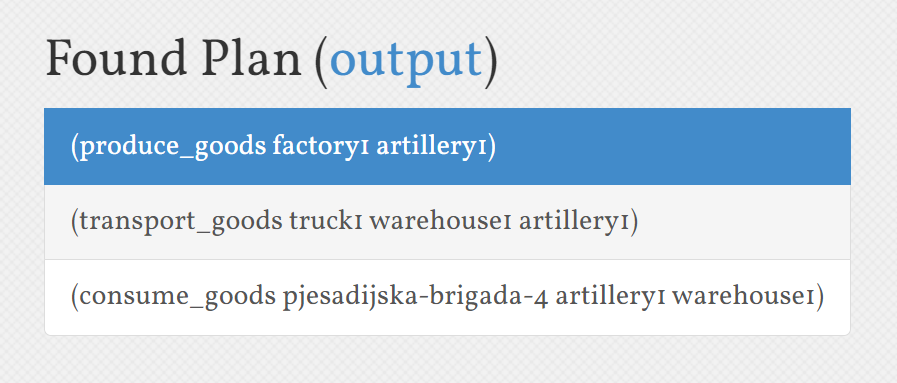
\includegraphics[width=1\textwidth]{Plan1}}
\end{figure}
\noindent
Kao i očekivano, rješenje ovog problema je veoma jednostavno. Fabrika proizvodi artiljeriju, kamion je transportuje u skladiste, a pjesadijska brigada upotrebljava artiljeriju iz skladista. Kako smo uspjeli riješiti problem logistike na pojednostavljenom modelu, pređimo sada na složenji model problema.\\~\\

\Large
\noindent
\textbf{Model 2}
\\~\\
\normalsize 
U ovom modelu logistike Oružanih snaga BiH, dodati ćemo ostale jednostavne pješadijske brigade, dodane kamione, fabrike i skladišta.
\\~\\
\textbf{\textit{domain.pddl}}
\begin{verbatim}
(define (domain vojna-logistika-expanded)
    (:requirements :strips :typing :fluents)

    (:types
        division factory warehouse good truck
    )

    (:constants
        Pjesadijska-brigada-4 - division
        Pjesadijska-brigada-5 - division
        Pjesadijska-brigada-6 - division
        BINAS-DD Cajevac RZT Igman TRZ Orao Vitezit Pretis Kosmos BNT - factory
        Warehouse1 Warehouse2 Warehouse3 - warehouse
        Artillery1 Utility-equipment1 Telecommunication-equipment1  
            Ammunition1 Protective-gear1 Explosives1 Guns1 - good
        Truck1 Truck2 Truck3 Truck4 Truck5 Truck6 Truck7 Truck8 - truck
    )

    (:predicates
        (produced ?f - factory ?g - good)
        (transported ?t - truck ?w - warehouse ?g - good)
        (stored ?w - warehouse ?g - good)
        (consumed ?d - division ?g - good)
        (truck_available ?t - truck)
        (division_needs ?d - division ?g - good)
    )

    (:action produce_goods
        :parameters (?f - factory ?g - good)
        :precondition (not (produced ?f ?g))
        :effect (produced ?f ?g)
    )

    (:action transport_goods
        :parameters (?t - truck ?w - warehouse ?g - good)
        :precondition (and (produced BINAS-DD ?g) (truck_available ?t))
        :effect (and (transported ?t ?w ?g) (stored ?w ?g) (not (truck_available ?t)))
    )

    (:action consume_goods
        :parameters (?d - division ?g - good ?w - warehouse)
        :precondition (and (stored ?w ?g) (division_needs ?d ?g))
        :effect (consumed ?d ?g)
    )
)

\end{verbatim}

\noindent\textbf{\textit{problem.pddl}}
\begin{verbatim}
(define (problem expanded-logistics)
    (:domain vojna-logistika-expanded)

    (:objects
        Warehouse1 Warehouse2 Warehouse3 - warehouse
        Artillery1 Utility-equipment1 Telecommunication-equipment1 
            Ammunition1 Protective-gear1 Explosives1 Guns1 - good
        Truck1 Truck2 Truck3 Truck4 Truck5 Truck6 Truck7 Truck8 - truck
    )

    (:init
        (truck_available Truck1)
        (truck_available Truck2)
        (truck_available Truck3)
        (truck_available Truck4)
        (truck_available Truck5)
        (truck_available Truck6)
        (truck_available Truck7)
        (truck_available Truck8)

        (division_needs Pjesadijska-brigada-4 Artillery1)
        (division_needs Pjesadijska-brigada-4 Utility-equipment1)
        (division_needs Pjesadijska-brigada-4 Telecommunication-equipment1)
        (division_needs Pjesadijska-brigada-4 Ammunition1)
        (division_needs Pjesadijska-brigada-4 Protective-gear1)
        (division_needs Pjesadijska-brigada-4 Explosives1)
        (division_needs Pjesadijska-brigada-4 Guns1)
        
        (division_needs Pjesadijska-brigada-5 Artillery1)
        (division_needs Pjesadijska-brigada-5 Utility-equipment1)
        (division_needs Pjesadijska-brigada-5 Telecommunication-equipment1)
        (division_needs Pjesadijska-brigada-5 Ammunition1)
        (division_needs Pjesadijska-brigada-5 Protective-gear1)
        (division_needs Pjesadijska-brigada-5 Explosives1)
        (division_needs Pjesadijska-brigada-5 Guns1)
        
        (division_needs Pjesadijska-brigada-6 Artillery1)
        (division_needs Pjesadijska-brigada-6 Utility-equipment1)
        (division_needs Pjesadijska-brigada-6 Telecommunication-equipment1)
        (division_needs Pjesadijska-brigada-6 Ammunition1)
        (division_needs Pjesadijska-brigada-6 Protective-gear1)
        (division_needs Pjesadijska-brigada-6 Explosives1)
        (division_needs Pjesadijska-brigada-6 Guns1)

        (produced BINAS-DD Artillery1)
        (produced Cajevac Utility-equipment1)
        (produced RZT Telecommunication-equipment1)
        (produced Igman Ammunition1)
        (produced TRZ Protective-gear1)
        (produced Orao Explosives1)
        (produced Vitezit Guns1)
    )

    (:goal
        (and
            (consumed Pjesadijska-brigada-4 Artillery1)
            (consumed Pjesadijska-brigada-4 Utility-equipment1)
            (consumed Pjesadijska-brigada-4 Telecommunication-equipment1)
            (consumed Pjesadijska-brigada-4 Ammunition1)
            (consumed Pjesadijska-brigada-4 Protective-gear1)
            (consumed Pjesadijska-brigada-4 Explosives1)
            (consumed Pjesadijska-brigada-4 Guns1)
            
            (consumed Pjesadijska-brigada-5 Artillery1)
            (consumed Pjesadijska-brigada-5 Utility-equipment1)
            (consumed Pjesadijska-brigada-5 Telecommunication-equipment1)
            (consumed Pjesadijska-brigada-5 Ammunition1)
            (consumed Pjesadijska-brigada-5 Protective-gear1)
            (consumed Pjesadijska-brigada-5 Explosives1)
            (consumed Pjesadijska-brigada-5 Guns1)
            
            (consumed Pjesadijska-brigada-6 Artillery1)
            (consumed Pjesadijska-brigada-6 Utility-equipment1)
            (consumed Pjesadijska-brigada-6 Telecommunication-equipment1)
            (consumed Pjesadijska-brigada-6 Ammunition1)
            (consumed Pjesadijska-brigada-6 Protective-gear1)
            (consumed Pjesadijska-brigada-6 Explosives1)
            (consumed Pjesadijska-brigada-6 Guns1)
        )
    )
)

\end{verbatim}
\begin{figure}[H] 
  \noindent\makebox[\textwidth]{%
  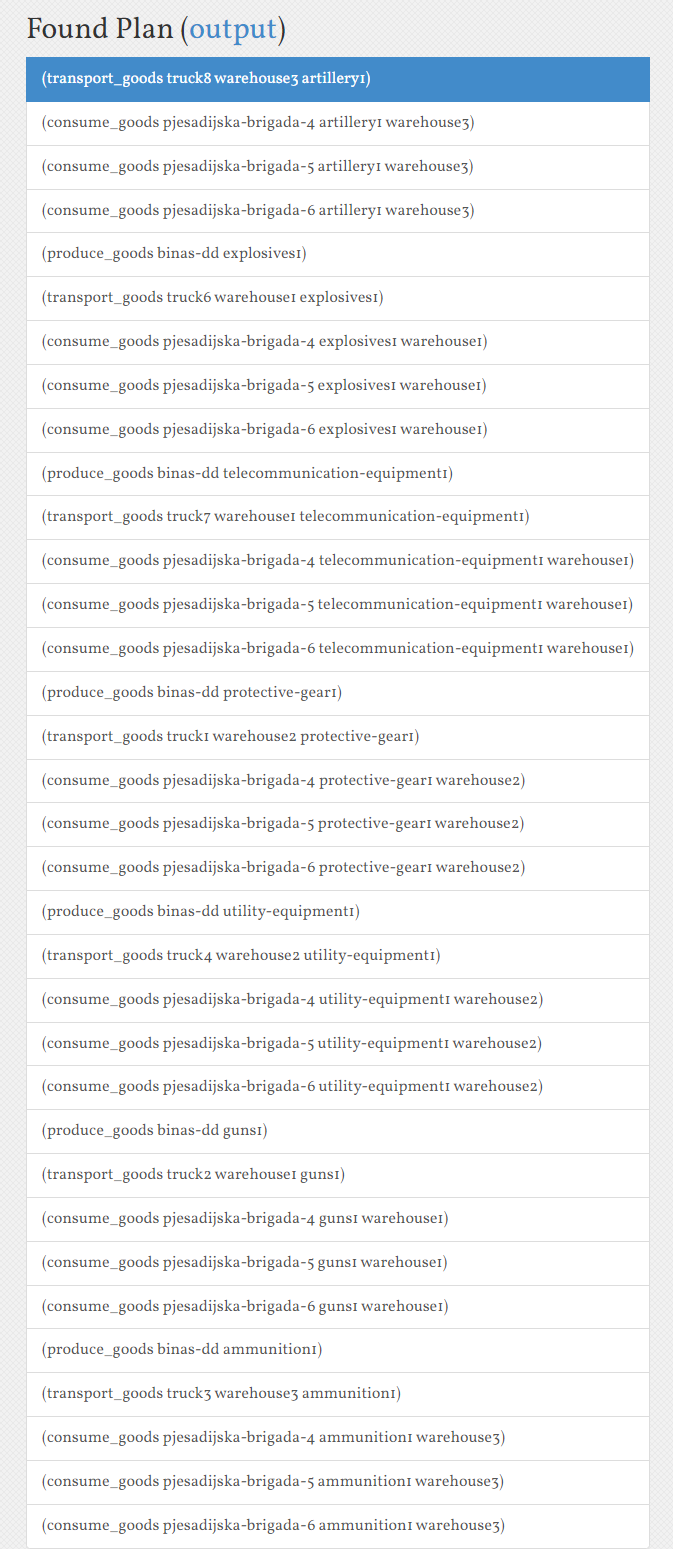
\includegraphics[width=0.7\textwidth]{Plan2}}
\end{figure}

\noindent
Rješenje ovog modela, iako značajno duže, nije mnogo kompleksije od prvog. Ukoliko se neka oprema već nalazi u skladištu, jedna po jedna pješadijska brigada je uzima za sebe. Ukoliko nije, čeka se da fabrika proizvede opremu, kamionima se prenosi u jedno od skladišta, te ih konačno opet jedna po jedna brigada uzima.\\~\\

\Large
\noindent
\textbf{Finalni model}
\\~\\
\normalsize 
Finalni model predstavlja najkompleksniji od svih dosadasnjih modela, te i ultimativno rješenje originalno postavljenog problema. Data su tri skladišta, široki izbor opreme, osam kamiona i deset fabrika koje proizvode svu opremu. Određena oprema se uvozi, dok se ostatak proizvodi u BiH. Skladišta su na početku prazna a svim brigadama je potreba oprema i vozila.
\\~\\
\textbf{\textit{domain.pddl}}
\begin{verbatim}
(define (domain vojna-logistika-final)
    (:requirements :strips :typing :fluents)

    (:types
        division factory warehouse good truck armored-cars aircraft
    )

    (:constants
        Pjesadijska-brigada-4 - division
        Pjesadijska-brigada-5 - division
        Pjesadijska-brigada-6 - division
        Brigada-takticke-podrske - division
        Brigada-zracnih-snaga - division
        BINAS-DD Cajevac RZT Igman TRZ Orao Vitezit Pretis Kosmos BNT - factory
        Skladiste1 Skladiste2 Skladiste3 - warehouse
        Artiljerija Dodatna_Oprema Telekomunikacijska_Oprema Municija Zastitna_Oprema 
            Eksplozivi Puske Napredni_Explozivi Oklopno_Vozilo Tenk Borbeni_Avion 
            Avion_Presretac Helikopter - good
        Kamion1 Kamion2 Kamion3 Kamion4 Kamion5 Kamion6 Kamion7 Kamion8 - truck
    )

    (:predicates
        (produced ?f - factory ?g - good)
        (imported ?g - good)
        (transported ?t - truck ?w - warehouse ?g - good)
        (stored ?w - warehouse ?g - good)
        (consumed ?d - division ?g - good)
        (truck_available ?t - truck)
        (division_needs ?d - division ?g - good)
        (good_producible ?g - good)
        (produced_and_stored ?w - warehouse ?g - good)
    )

    (:action produce_goods
        :parameters (?f - factory ?g - good ?w - warehouse)
        :precondition (and (good_producible ?g) (not (produced ?f ?g)))
        :effect (and (produced ?f ?g) (stored ?w ?g) (produced_and_stored ?w ?g))
    )

    (:action import_goods
        :parameters (?g - good ?w - warehouse)
        :precondition (and (imported ?g) (not (stored ?w ?g)))
        :effect (and (imported ?g) (stored ?w ?g))
    )

    (:action transport_goods
        :parameters (?t - truck ?w - warehouse ?g - good)
        :precondition (and (or (imported ?g) (exists (?f - factory) 
            (produced ?f ?g))) (truck_available ?t))
        :effect (and (transported ?t ?w ?g) (stored ?w ?g) (not (truck_available ?t)))
    )

    (:action consume_goods
        :parameters (?d - division ?g - good ?w - warehouse)
        :precondition (and (stored ?w ?g) (division_needs ?d ?g))
        :effect (consumed ?d ?g)
    )
)

\end{verbatim}

\noindent
\textbf{\textit{problem.pddl}}
\begin{verbatim}
(define (problem final-logistics)
    (:domain vojna-logistika-final)

    (:objects
        Skladiste1 Skladiste2 Skladiste3 - warehouse
        Artiljerija Dodatna_Oprema Telekomunikacijska_Oprema Municija Zastitna_Oprema 
            Eksplozivi Puske Napredni_Eksplozivi Oklopna_Vozila Tenkovi Borbeni_Avioni 
            Avioni_Presretaci Helikopteri - good
        Kamion1 Kamion2 Kamion3 Kamion4 Kamion5 Kamion6 Kamion7 Kamion8 - truck
        BINAS-DD Cajevac RZT Igman TRZ Orao Vitezit Pretis Kosmos BNT - factory
    )

    (:init
        ;; Kamioni
        (truck_available Kamion1)
        (truck_available Kamion2)
        (truck_available Kamion3)
        (truck_available Kamion4)
        (truck_available Kamion5)
        (truck_available Kamion6)
        (truck_available Kamion7)
        (truck_available Kamion8)

        ;; Oprema koja se moze proizvoditi
        (good_producible Artiljerija)
        (good_producible Dodatna_Oprema)
        (good_producible Telekomunikacijska_Oprema)
        (good_producible Municija)
        (good_producible Zastitna_Oprema)
        (good_producible Eksplozivi)
        (good_producible Puske)

        ;; Uvozimo sve
        (imported Napredni_Eksplozivi)
        (imported Oklopna_Vozila)
        (imported Tenkovi)
        (imported Borbeni_Avioni)
        (imported Avioni_Presretaci)
        (imported Helikopteri)

        ;; Sva skladista prazna
        (not (stored Skladiste1 Artiljerija))
        (not (stored Skladiste1 Dodatna_Oprema))
        (not (stored Skladiste1 Telekomunikacijska_Oprema))
        (not (stored Skladiste1 Municija))
        (not (stored Skladiste1 Zastitna_Oprema))
        (not (stored Skladiste1 Eksplozivi))
        (not (stored Skladiste1 Puske))
        (not (stored Skladiste1 Napredni_Eksplozivi))
        (not (stored Skladiste1 Oklopna_Vozila))
        (not (stored Skladiste1 Tenkovi))
        (not (stored Skladiste1 Borbeni_Avioni))
        (not (stored Skladiste1 Avioni_Presretaci))
        (not (stored Skladiste1 Helikopteri))

        (not (stored Skladiste2 Artiljerija))
        (not (stored Skladiste2 Dodatna_Oprema))
        (not (stored Skladiste2 Telekomunikacijska_Oprema))
        (not (stored Skladiste2 Municija))
        (not (stored Skladiste2 Zastitna_Oprema))
        (not (stored Skladiste2 Eksplozivi))
        (not (stored Skladiste2 Puske))
        (not (stored Skladiste2 Napredni_Eksplozivi))
        (not (stored Skladiste2 Oklopna_Vozila))
        (not (stored Skladiste2 Tenkovi))
        (not (stored Skladiste2 Borbeni_Avioni))
        (not (stored Skladiste2 Avioni_Presretaci))
        (not (stored Skladiste2 Helikopteri))

        (not (stored Skladiste3 Artiljerija))
        (not (stored Skladiste3 Dodatna_Oprema))
        (not (stored Skladiste3 Telekomunikacijska_Oprema))
        (not (stored Skladiste3 Municija))
        (not (stored Skladiste3 Zastitna_Oprema))
        (not (stored Skladiste3 Eksplozivi))
        (not (stored Skladiste3 Puske))
        (not (stored Skladiste3 Napredni_Eksplozivi))
        (not (stored Skladiste3 Oklopna_Vozila))
        (not (stored Skladiste3 Tenkovi))
        (not (stored Skladiste3 Borbeni_Avioni))
        (not (stored Skladiste3 Avioni_Presretaci))
        (not (stored Skladiste3 Helikopteri))

        ;; Postavljamo sta brigade trebaju
        (division_needs Pjesadijska-brigada-4 Artiljerija)
        (division_needs Pjesadijska-brigada-4 Dodatna_Oprema)
        (division_needs Pjesadijska-brigada-4 Telekomunikacijska_Oprema)
        (division_needs Pjesadijska-brigada-4 Municija)
        (division_needs Pjesadijska-brigada-4 Zastitna_Oprema)
        (division_needs Pjesadijska-brigada-4 Eksplozivi)
        (division_needs Pjesadijska-brigada-4 Oklopna_Vozila)
        (division_needs Pjesadijska-brigada-4 Tenkovi)
        (division_needs Pjesadijska-brigada-4 Puske)
        
        (division_needs Pjesadijska-brigada-5 Artiljerija)
        (division_needs Pjesadijska-brigada-5 Dodatna_Oprema)
        (division_needs Pjesadijska-brigada-5 Telekomunikacijska_Oprema)
        (division_needs Pjesadijska-brigada-5 Municija)
        (division_needs Pjesadijska-brigada-5 Zastitna_Oprema)
        (division_needs Pjesadijska-brigada-5 Eksplozivi)
        (division_needs Pjesadijska-brigada-5 Oklopna_Vozila)
        (division_needs Pjesadijska-brigada-5 Tenkovi)
        (division_needs Pjesadijska-brigada-5 Puske)
        
        (division_needs Pjesadijska-brigada-6 Artiljerija)
        (division_needs Pjesadijska-brigada-6 Dodatna_Oprema)
        (division_needs Pjesadijska-brigada-6 Telekomunikacijska_Oprema)
        (division_needs Pjesadijska-brigada-6 Municija)
        (division_needs Pjesadijska-brigada-6 Zastitna_Oprema)
        (division_needs Pjesadijska-brigada-6 Eksplozivi)
        (division_needs Pjesadijska-brigada-6 Oklopna_Vozila)
        (division_needs Pjesadijska-brigada-6 Tenkovi)
        (division_needs Pjesadijska-brigada-6 Puske)
        
        (division_needs Brigada-zracnih-snaga Borbeni_Avioni)
        (division_needs Brigada-zracnih-snaga Avioni_Presretaci)
        (division_needs Brigada-zracnih-snaga Helikopteri)
        
        (division_needs Brigada-takticke-podrske Dodatna_Oprema)
        (division_needs Brigada-takticke-podrske Telekomunikacijska_Oprema)
        (division_needs Brigada-takticke-podrske Zastitna_Oprema)
        (division_needs Brigada-takticke-podrske Napredni_Eksplozivi)
    )

    (:goal
        (and
            (consumed Pjesadijska-brigada-4 Artiljerija)
            (consumed Pjesadijska-brigada-4 Dodatna_Oprema)
            (consumed Pjesadijska-brigada-4 Telekomunikacijska_Oprema)
            (consumed Pjesadijska-brigada-4 Municija)
            (consumed Pjesadijska-brigada-4 Zastitna_Oprema)
            (consumed Pjesadijska-brigada-4 Eksplozivi)
            (consumed Pjesadijska-brigada-4 Oklopna_Vozila)
            (consumed Pjesadijska-brigada-4 Tenkovi)
            (consumed Pjesadijska-brigada-4 Puske)
            
            (consumed Pjesadijska-brigada-5 Artiljerija)
            (consumed Pjesadijska-brigada-5 Dodatna_Oprema)
            (consumed Pjesadijska-brigada-5 Telekomunikacijska_Oprema)
            (consumed Pjesadijska-brigada-5 Municija)
            (consumed Pjesadijska-brigada-5 Zastitna_Oprema)
            (consumed Pjesadijska-brigada-5 Eksplozivi)
            (consumed Pjesadijska-brigada-5 Oklopna_Vozila)
            (consumed Pjesadijska-brigada-5 Tenkovi)
            (consumed Pjesadijska-brigada-5 Puske)
            
            (consumed Pjesadijska-brigada-6 Artiljerija)
            (consumed Pjesadijska-brigada-6 Dodatna_Oprema)
            (consumed Pjesadijska-brigada-6 Telekomunikacijska_Oprema)
            (consumed Pjesadijska-brigada-6 Municija)
            (consumed Pjesadijska-brigada-6 Zastitna_Oprema)
            (consumed Pjesadijska-brigada-6 Eksplozivi)
            (consumed Pjesadijska-brigada-6 Oklopna_Vozila)
            (consumed Pjesadijska-brigada-6 Tenkovi)
            (consumed Pjesadijska-brigada-6 Puske)
            
            (consumed Brigada-takticke-podrske Dodatna_Oprema)
            (consumed Brigada-takticke-podrske Telekomunikacijska_Oprema)
            (consumed Brigada-takticke-podrske Zastitna_Oprema)
            (consumed Brigada-takticke-podrske Napredni_Eksplozivi)
            
            (consumed Brigada-zracnih-snaga Borbeni_Avioni)
            (consumed Brigada-zracnih-snaga Avioni_Presretaci)
            (consumed Brigada-zracnih-snaga Helikopteri)
        )
    )
)
\end{verbatim}

\begin{figure}[H]
  \centering
  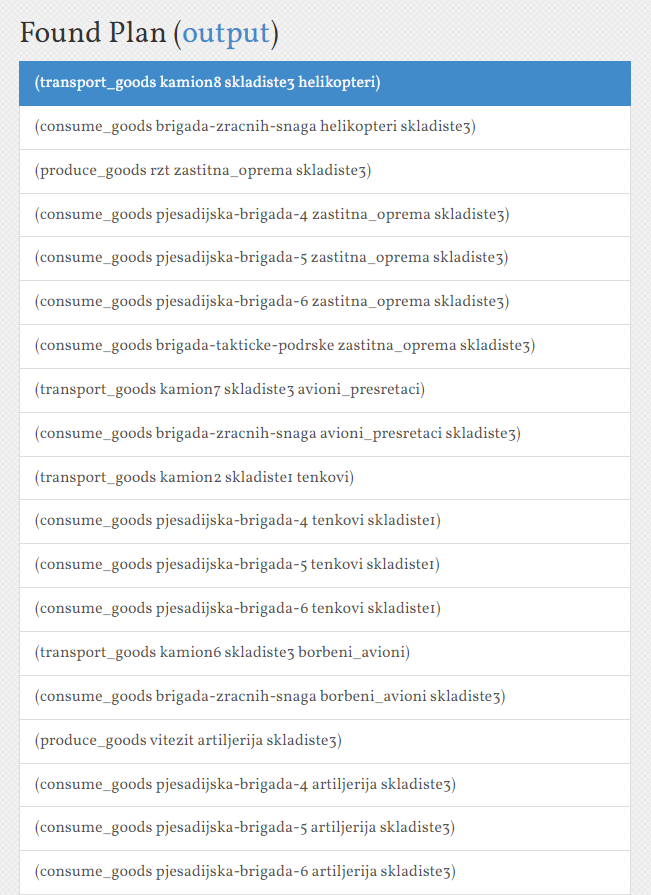
\includegraphics[width=0.7\textwidth]{Plan3_1}
\end{figure}

\clearpage
\begin{figure}[H]
  \centering
  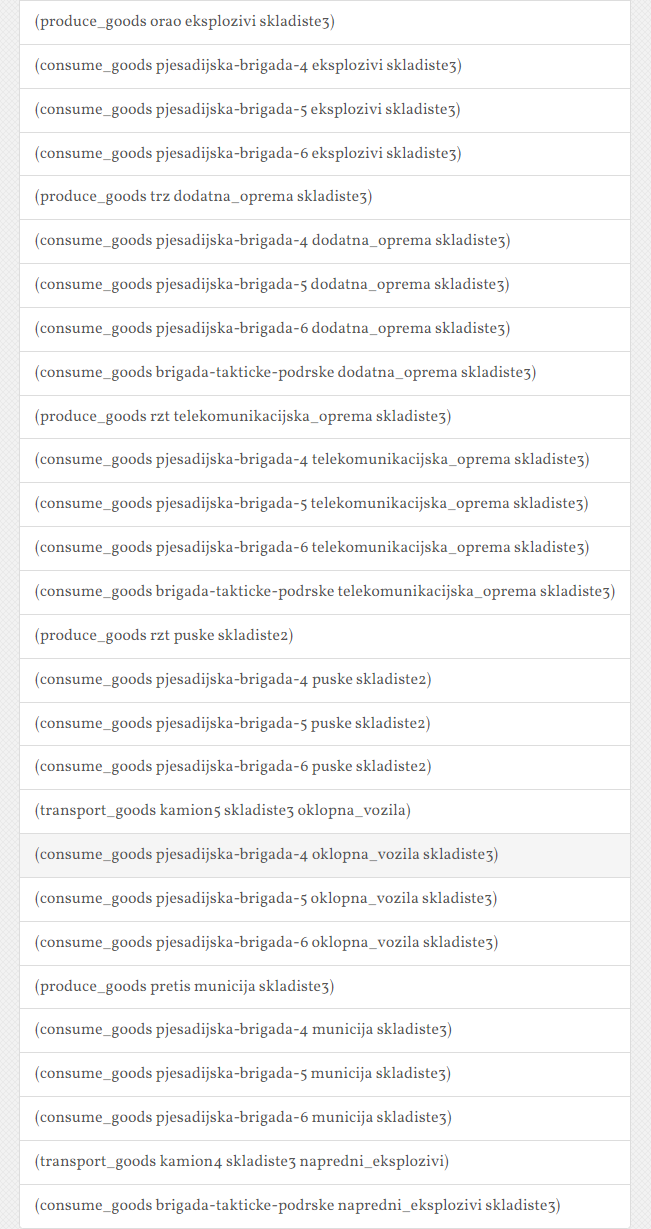
\includegraphics[width=0.7\textwidth]{Plan3_2}
\end{figure}

\subsection{Rezultati}
Za početak se uzima da je sva operma koja se uvozi već uvezena i nalazi se u skladištima. Helikopteri, koji će biti korišteni od strane brigade zračnih snaga iz skladišta 3, će biti transportovani jednim od kamiona do njega. Ako nastavimo dalje analizirati rješenje, vidjet ćemo da se dodatna oprema proizvodi u fabrici TRZ i smješta u skladištu 3, pri čemu sama dodatna oprema predstavlja bitan faktor, još bitniji ako je nema. Naravno, dodatnu opremu će koristiti sve pješadijske brigade, kao i brigada taktičke podrške. Također tenkovi, borbeni avioni i oklopna vozila, se transportuju pomoću kamiona i bit će korišteni od strane pojedinih pješadijskih brigada, u zavisnosti od toga za šta su tačno namijenjene. Što se tiče zaštitne opreme, ono će se proizvoditi u fabrici RZT, bit će smještena u skladište 2, te će biti korištena od strane svih pješadijskih brigada. Artiljerija će se proizvoditi u fabrici Vitezit, skladištiti u skladištu 3 i bit će korištena, također, od strane svih pješadijskih brigada. Što se tiče sad telekomunikacijske opreme, za njenu proizvodnju će također biti zadužena firma RZT, a procedura korištenja i skladištenja je ista kao i kod ostalih. Slično je i sa municijom koja će se proizvoditi u firmi Pretis, te i svom ostalom opremom.


\section{Zaključak}
U ovom radu smo se bavili modeliranjem logističkog sistema oružanih snaga Bosne i Hercegovine koristeći PDDL jezik. Kroz analizu i eksperimentisanje, došli smo do nekoliko ključnih zaključaka. Prvo, logistika se pokazala kao ključni element za operativnu efikasnost oružanih snaga. Bez adekvatne logističke podrške, sve operacije bi bile znatno otežane, što bi moglo dovesti do ozbiljnih posljedica na terenu.\\\\
Prikupljanje tačnih i pouzdanih podataka o logističkom sistemu oružanih snaga BiH pokazalo se kao izazovan zadatak zbog ograničenog pristupa informacijama. To nas je prisililo da donosimo određene pretpostavke koje su bile nužne za dalje modeliranje. Testiranje je pokazalo da je iterativni pristup, koji uključuje testiranje jednostavnijih modela prije nego što se pređe na složenije, ključ za efikasan razvoj konačnog modela. Ovaj pristup omogućava bržu identifikaciju i ispravku grešaka, kao i bolje razumijevanje problema i mogućih rješenja. 
\\\\
Iako je PDDL moćan alat za manja logička planiranja sa manje promenljivih, pokazalo se da nije najidealniji za realna i kompleksna logička planiranja. Tokom rada, više puta smo pokušavali da uključimo faktore poput goriva, nadopune i potrošnje goriva. Međutim, često se dešavalo da sistem prepoznaje postojanje rješenja, ali su ona bila prevelika ili ih je bilo previše da bi se mogla prikazati. Ovo ukazuje na ograničenja PDDL jezika za kompleksnije scenarije.\\\\
Uprkos nedostatku vremena, ovaj rad je pružio solidne temelje za dalja istraživanja, ali preostaje još mnogo posla. Dalje istraživanje bi trebalo uključivati testiranje novih modela i implementaciju predloženih unapređenja u stvarnim uslovima, te brojne druge stavke koje bi se uspješno mogle implementirati, iako nam je domen podataka ograničen. Uspješno smo modelirali osnovne elemente logističkog sistema BiH koristeći PDDL i testirali nekoliko od mnogih scenarija koji su nam pomogli da identifikujemo ključne probleme i potencijalna unapređenja. Isto tako, fokus bismo uputili na detaljnije prikupljanje realnih podataka, tj. dosta više bismo se obazirali na realni scenarij. Pored toga uključuli bismo i terenske studije i saradnju sa relevantnim vojnim strukturama. Također, istražili bismo naprednije tehnike optimizacije i simulacije, te integrisali dodatne varijable poput vremenskih uslova, geografske složenosti i različitih scenarija hitnih situacija. Sve ove dodatne aktivnosti bi pomogle u kreiranju još realističnijeg i efikasnijeg modela logističkog sistema oružanih snaga Bosne i Hercegovine.
\section{Doprinos članova tima}
\begin{itemize}
    \item \textbf{Uvod} - Irhad Žiga, Kerim Hajdar
    \item \textbf{Predloženo rješenje} - Vedad Gaštan, Aldin Velić
    \item \textbf{Zaključak} - Kerim Hajdar, Irhad Žiga
\end{itemize}
\textbf{Napomena}: Emin Šemić nije učestvovao u izradi ove zadaće !
\end{document}
